% \documentclass[a4paper]{article}
% \usepackage{graphicx}
% \usepackage{caption}
% \usepackage{subcaption}
% \begin{document}


\section{Results from applying homomorphic filtering}
	This section will present the results of applying homomorphic filtering (HF)
	on an image. Also provided is some experiments with different images
	and filters not used in the book, as to test if this method could yield
	better or worse results in different types of information depicted.
	\subsection{Results on the image provided with the project}
		The image provided with the project depicts a forest scenery, %include picture
		as seen in figure~\ref{fig:original}.
		\begin{figure}[h!]
			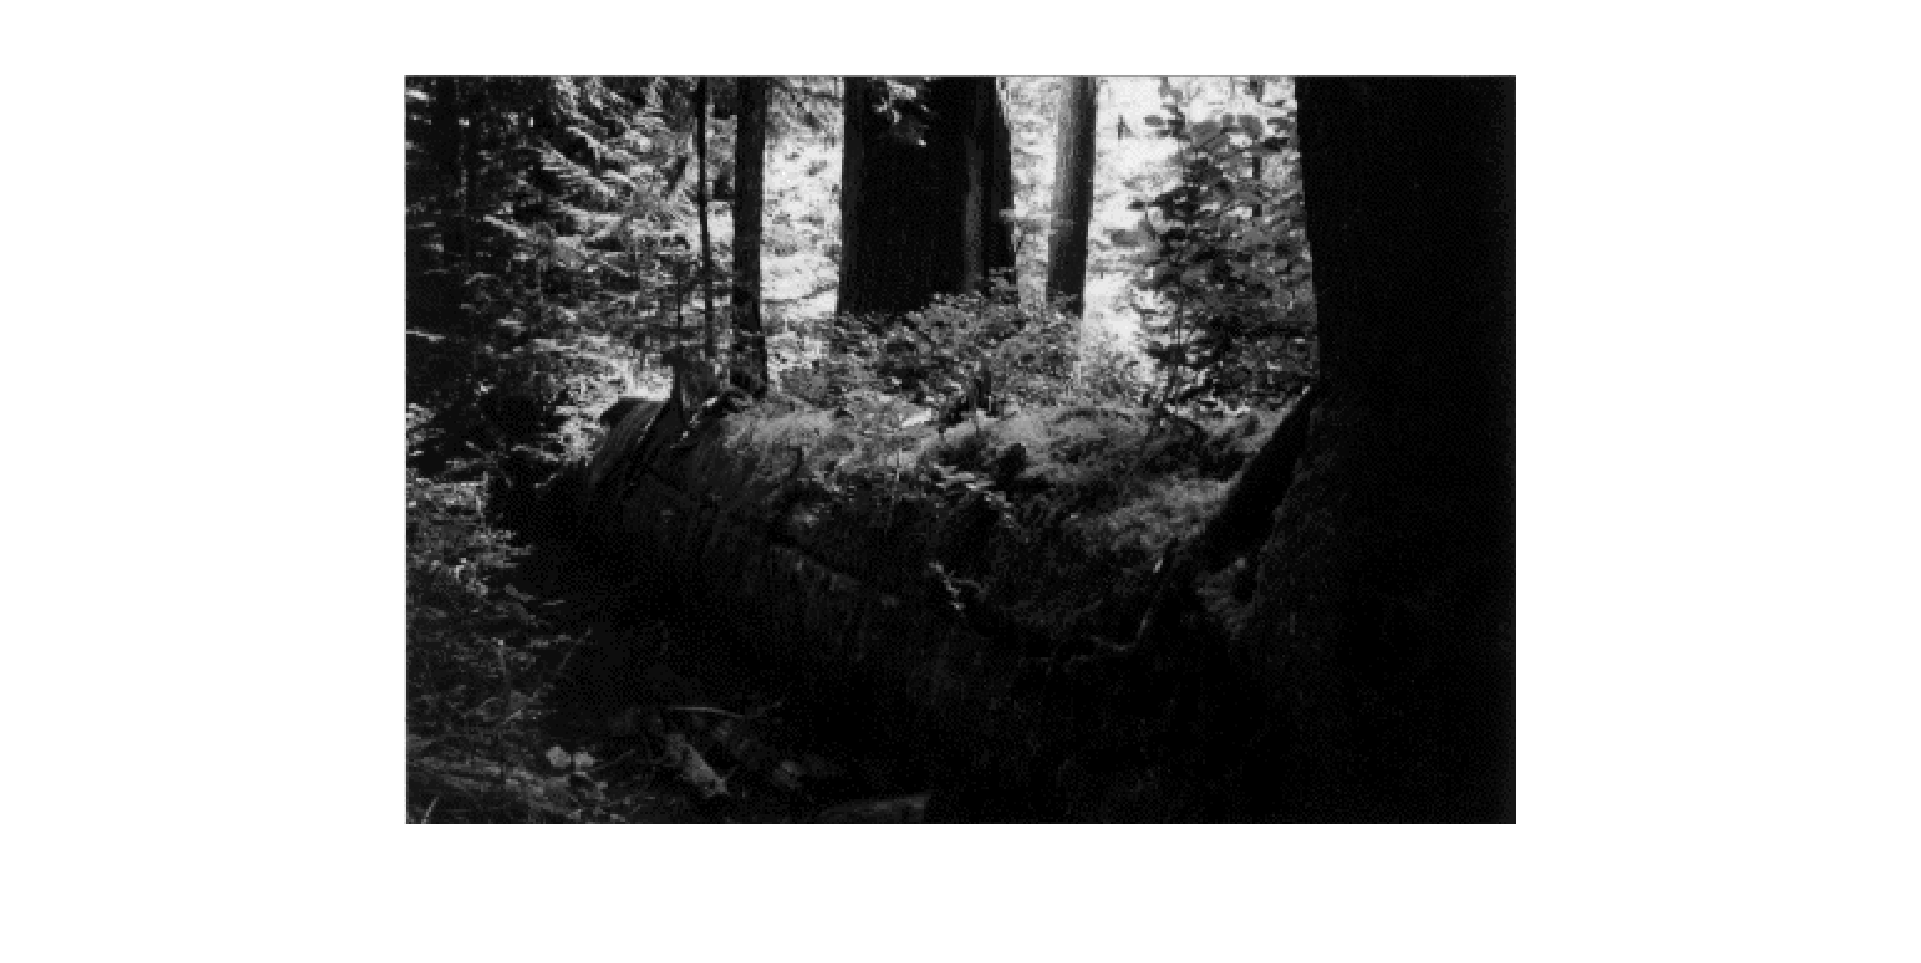
\includegraphics[width=\textwidth]{pics/orig_pic.png}
			\caption{The original picture, depicting a forest scenery}
			\label{fig:original}		
		\end{figure}		
		
		 %Har väl inga direkta större
		% inslag av kraftig illumination
		
%		The filter first used in this project was (as mentioned above)
%		the variant of the gaussian high-pass filter, detailed in the course book on pp. 314; 
		%
%		\begin{equation}
%		\label{eqn:gaussian_filter}
%			H(u,v) = \left( \gamma_H - \gamma_L \right) \left[ 1 - e^{-c \left[D^2(u,v)/D_0^2\right]}\right] + \gamma_L 
%		\end{equation}
		 %
		The filter in Eqn.~\ref{eqn:gaussian_filter} has the additional $\gamma$-parameters added in order to tweak
		the filter in regard to illumination and reflection. The $\gamma_L$ parameter
		will define the amount of suppression of the low frequencies (illumination); a lower $\gamma_L$
		will suppress low frequencies, which can be seen in figure~\ref{fig:low_freq_supp}.
		Figure~\ref{fig:low_freq_supp} shows how this setting enhances the information hidden 
		in the low frequencies, especially in the darker areas.
		Noteworthy is also that noise gets amplified as the lower frequencies gets suppressed, as can
		be seen in the lower part of the ridge in the center of figure~\ref{fig:low_freq_supp}.
		\begin{figure}[h!]
		\centering
		\begin{subfigure}[b]{0.5\textwidth}
			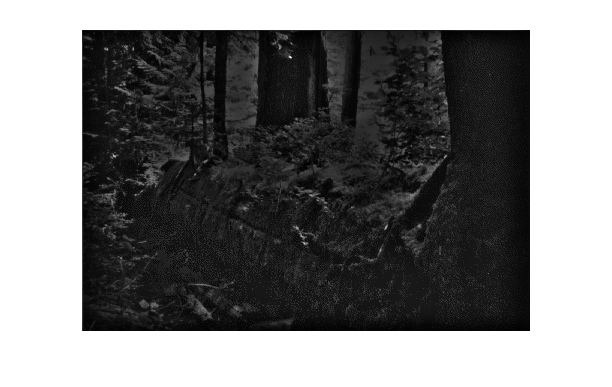
\includegraphics[width=\textwidth]{pics/suppressed_low_frequences.png}
			\caption{$\gamma_L = 0.01,~\gamma_H = 1$}
			\label{fig:low_freq_supp}
			\end{subfigure}%			
			\begin{subfigure}[b]{0.5\textwidth}
			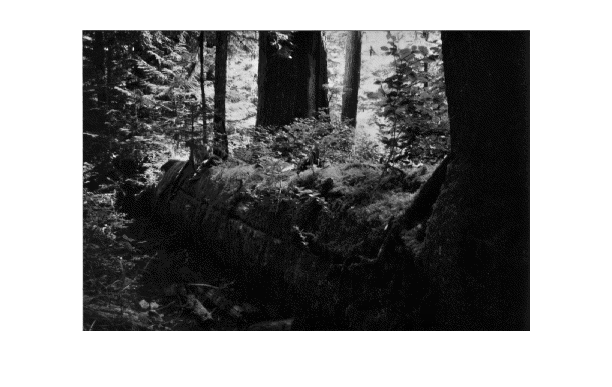
\includegraphics[width=\textwidth]{pics/non_suppressed_low_frequences.png}
			\caption{$\gamma_L = 0.8,~\gamma_H = 1$}
			\label{fig:low_freq_non_supp}
			\end{subfigure}
			\label{fig:various_low_gamma}
			\caption{The effect of changing $\gamma_L$}				
		\end{figure}		
		%
		\\
		\\
		A large value of the $\gamma_H$ parameter 
		will emphasize the high frequencies (reflection). As an example, 
		examine figure~\ref{fig:gamma_diff}.
		\begin{figure}[h!]
			\centering
			\begin{subfigure}[b]{0.5\textwidth}
				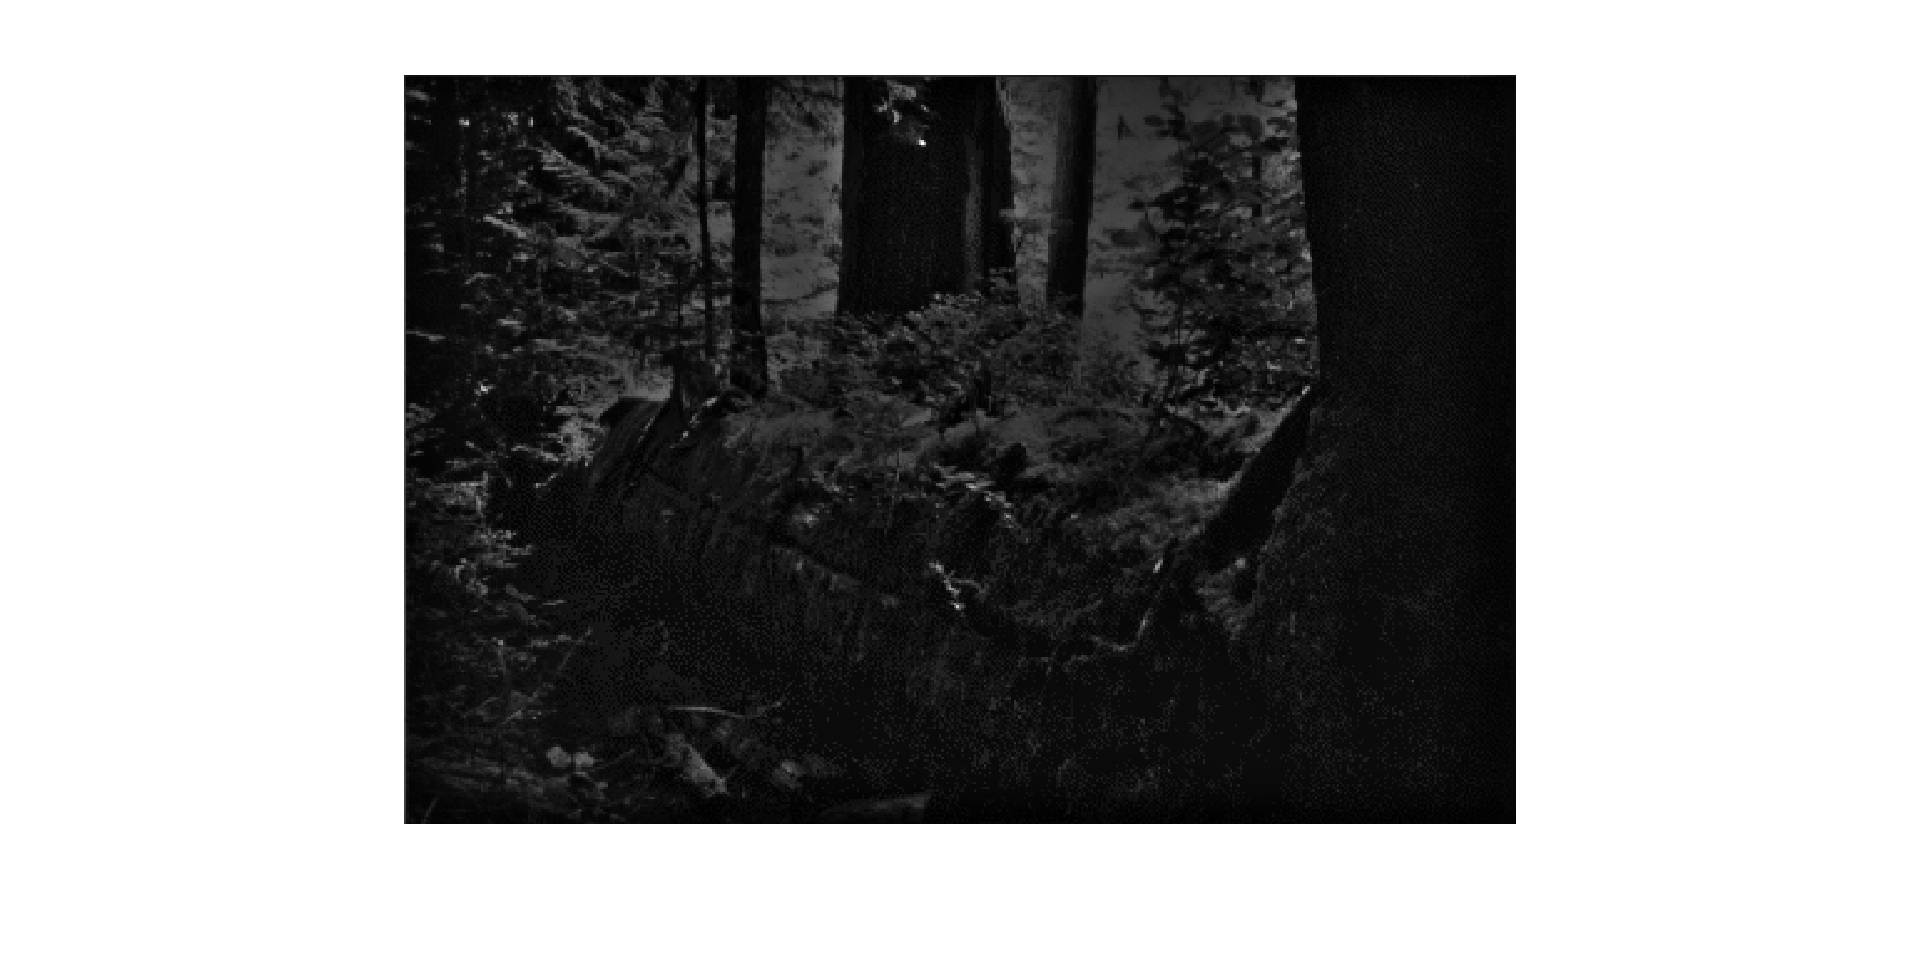
\includegraphics[width=\textwidth]{pics/non_emph_high_frequnces.png}
				\caption{$\gamma_L = 0.3,~\gamma_H = 1.2$}
				\label{fig:high_freq_non_emph}
			\end{subfigure}%
			\hfill	
			\begin{subfigure}[b]{0.5\textwidth}
				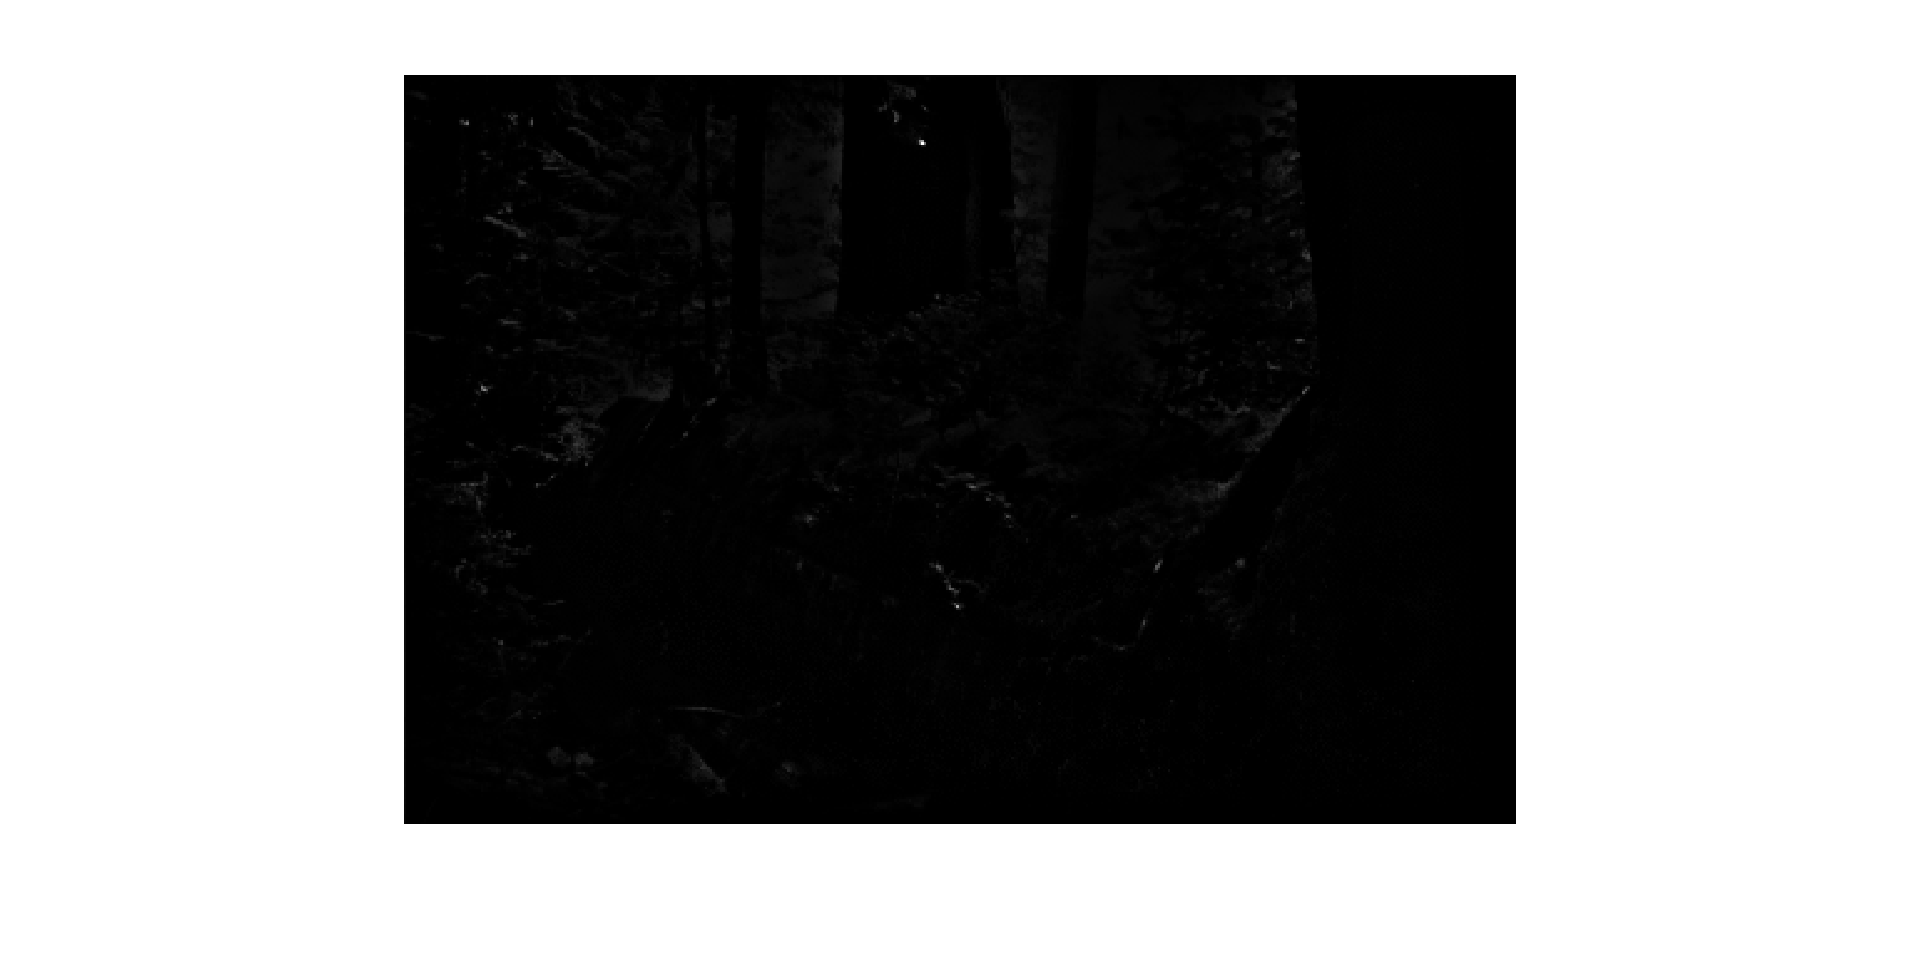
\includegraphics[width=\textwidth]{pics/emph_high_frequnces.png}
				\caption{$\gamma_L = 0.3,~\gamma_H = 2.5$}
				\label{fig:high_freq_emph}
			\end{subfigure}
			\label{fig:high_gamma}
		\caption{The effect of changing $\gamma_H$}				
		\end{figure}		
		One is able to see that the reflections gets emphasized and the overall
		image gets darker and more polarized. This can be seen clearly in the contrast from the
		tree trunk and the background, and in the white spots from the reflectant leaves.
		\\
		\\
		The third and final parameter is $D_0$, which controls the steepness of the filter.
		In practice, this means that a larger $D_0$ will produce an image with a more 
		narrow spectra of gray levels. The effect of this is visible in figure~\ref{fig:sigma}
		\begin{figure}[h!]
			\centering
			\begin{subfigure}[b]{0.5\textwidth}
				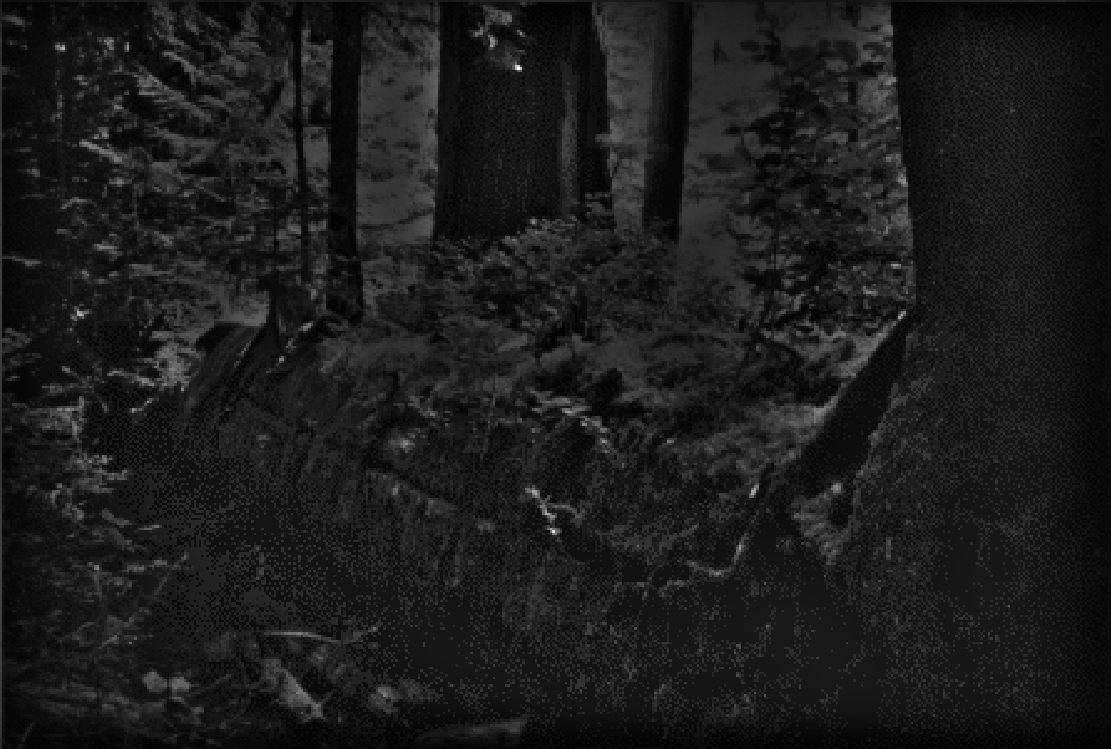
\includegraphics[width=\textwidth]{pics/low_sigma.png}
				\caption{$\gamma_L = 0,~\gamma_H = 1,~D_0 = 10$}
				\label{fig:low_sigma}
			\end{subfigure}%
			\begin{subfigure}[b]{0.5\textwidth}
				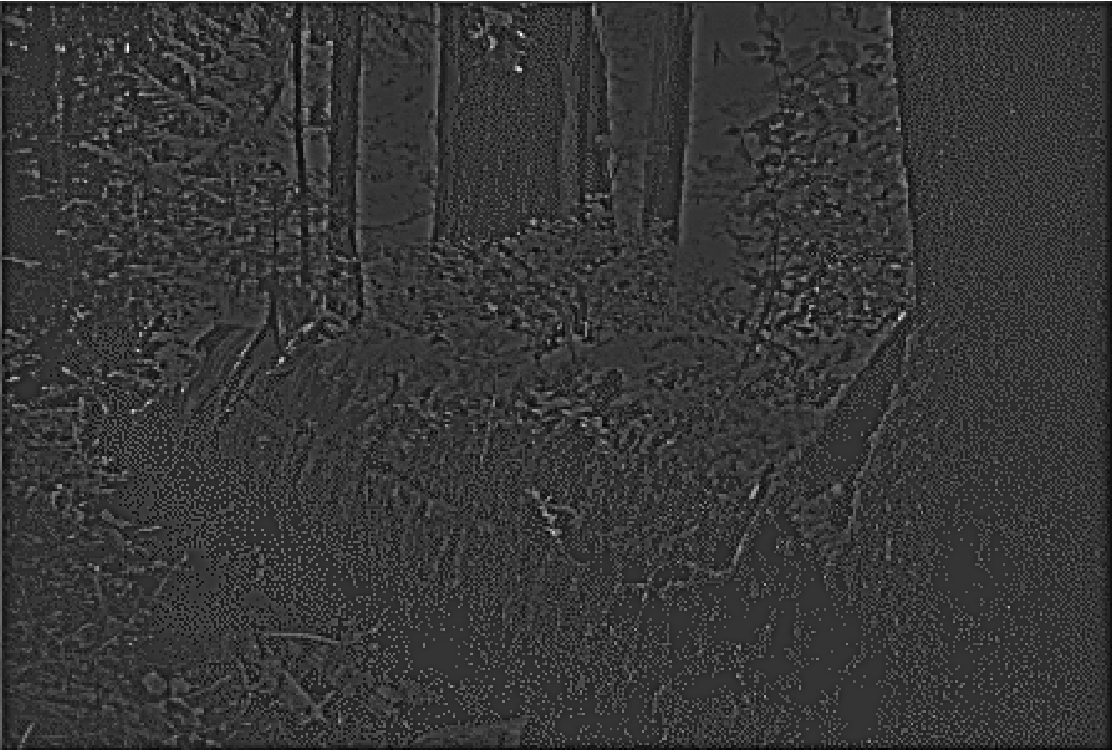
\includegraphics[width=\textwidth]{pics/high_sigma.png}
				\caption{$\gamma_L = 0,~\gamma_H = 1,~D_0 =80$}
				\label{fig:high_sigma}
			\end{subfigure}
			\label{fig:sigma}
			\begin{subfigure}[b]{0.5\textwidth}
				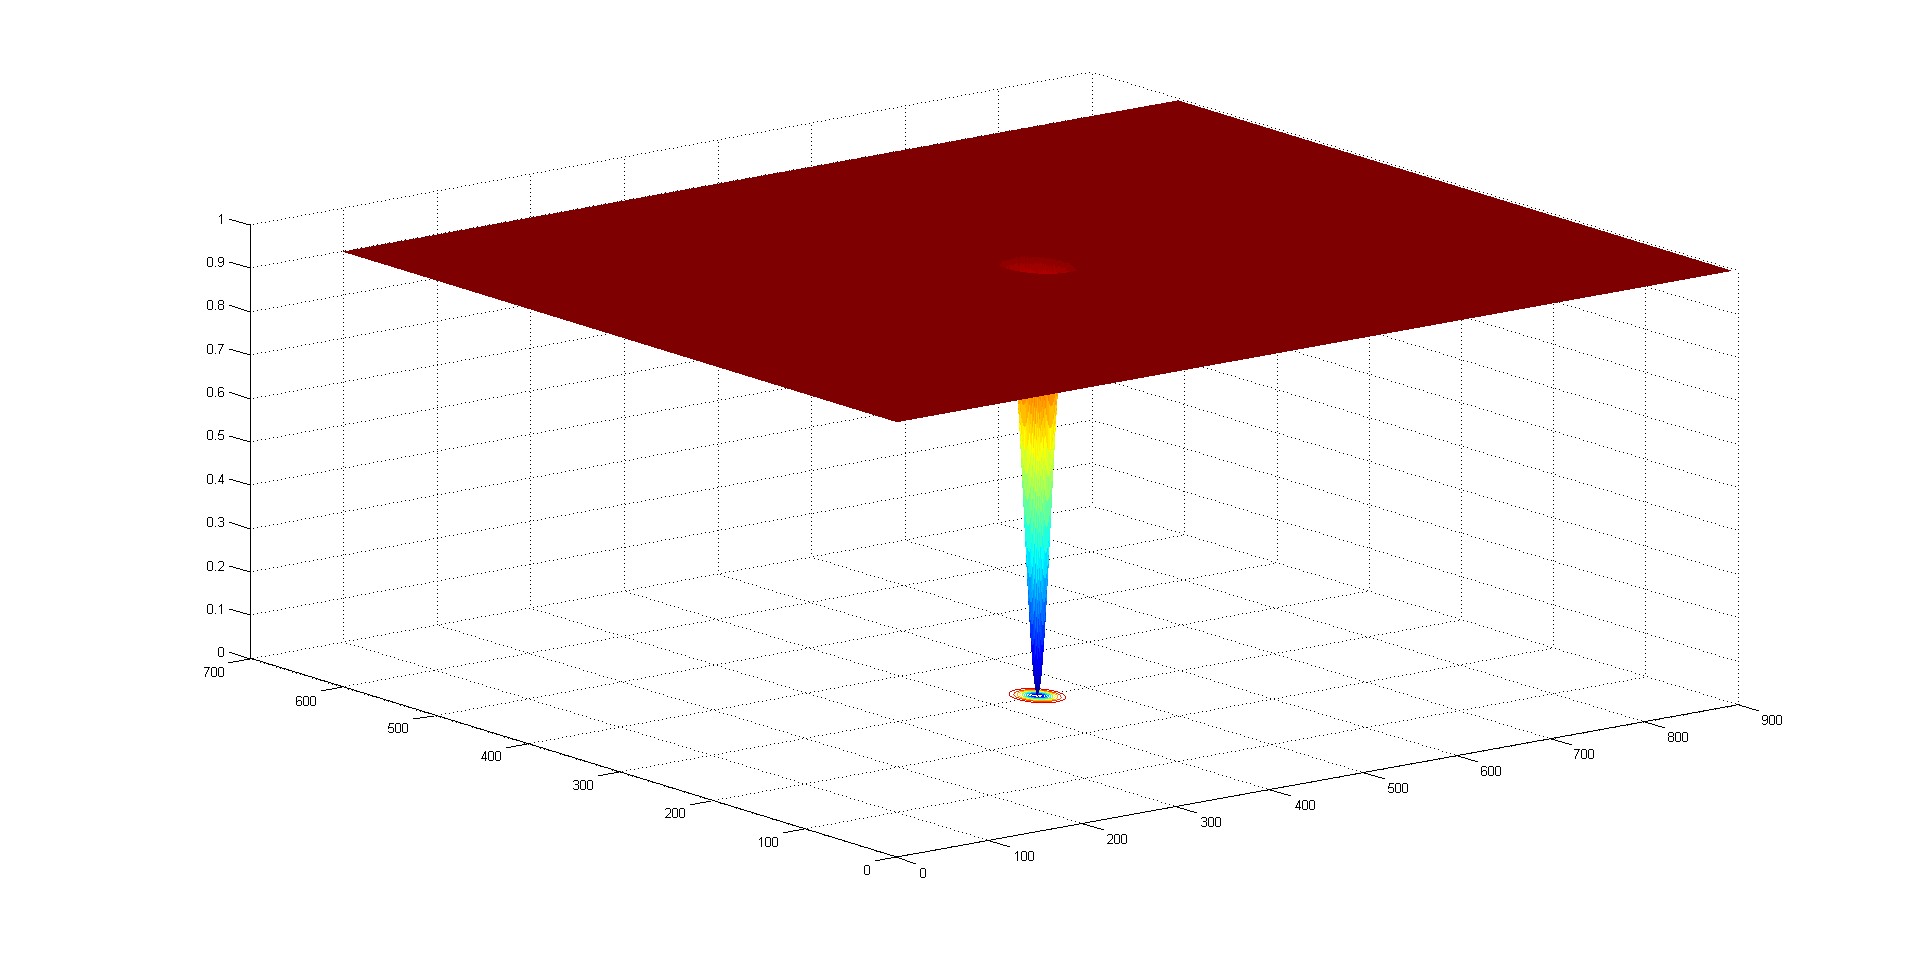
\includegraphics[width=\textwidth]{pics/low_sigma_filter.png}
				\caption{}
				\label{fig:low_sigma_filter}
			\end{subfigure}%
			\begin{subfigure}[b]{0.5\textwidth}
				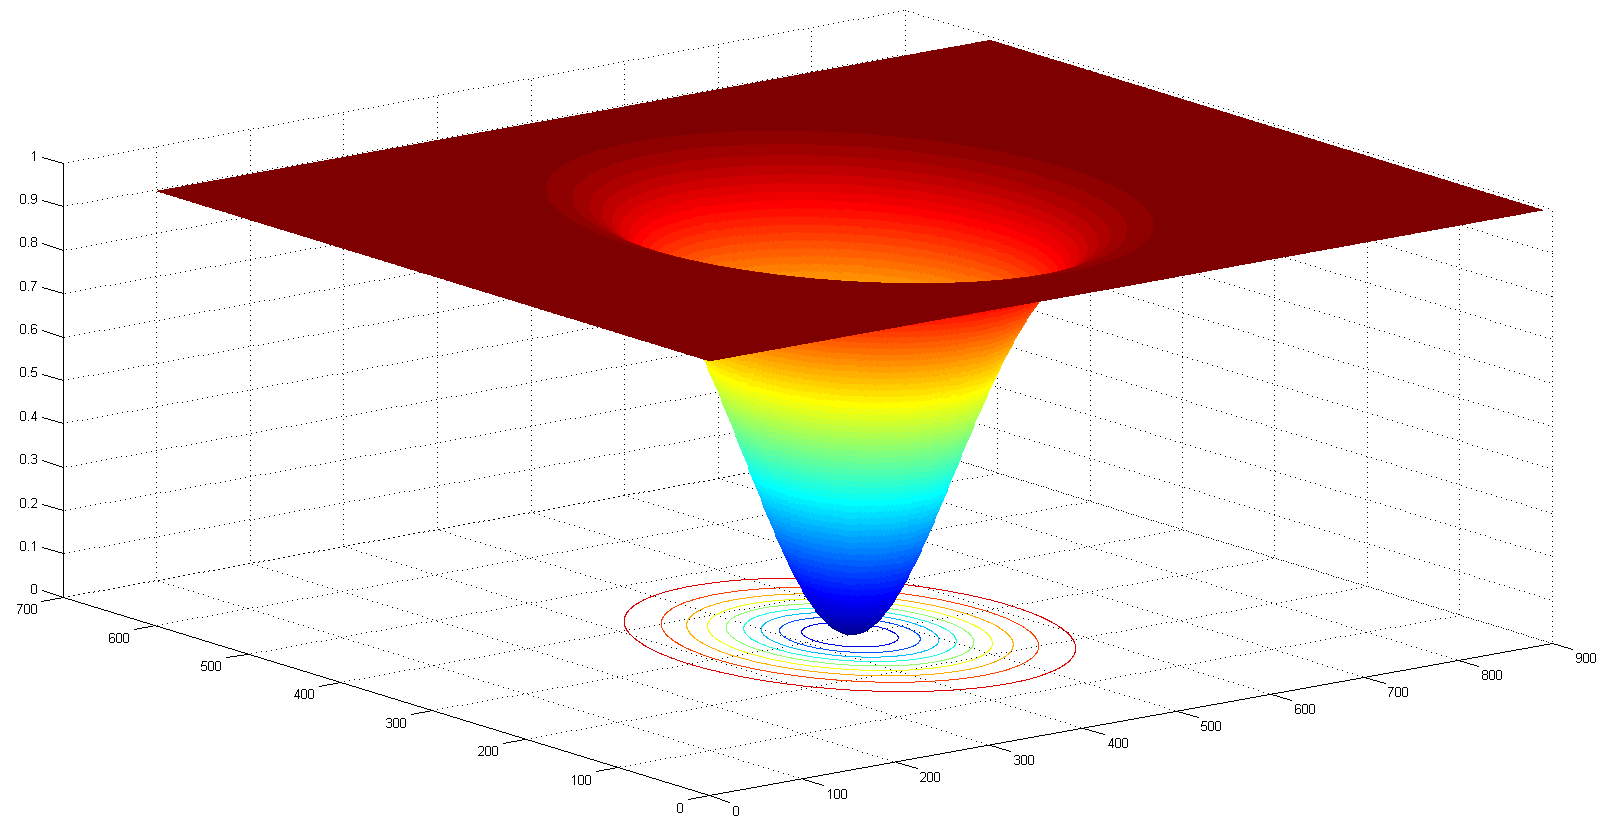
\includegraphics[width=\textwidth]{pics/high_sigma_filter.png}
				\caption{}
				\label{fig:high_sigma_filter}
			\end{subfigure}
			\label{fig:sigma}
		\caption{The effect of changing $D_0$, with the corresponding filter below each result}				
		\end{figure}
		with the corresponding filters. A very high $D_0$ is moving close to edge detection
		techniques,
		which can be very useful in areas such as computer vision, which is described in 
		the paper~\cite{Fan20111468}.\\
		\subsection{Conclusion}
		Various $\gamma_l$ and $\gamma_h$ paramaters has been tried out empirically with 
		various results. One has to ask oneself; What information should be extracted, and what 
		method performs best? When experimenting with emphasizing the reflections, the 
		general results was not very good. Usually the image got very dark with a few white
		spots from the highest frequencies, like in figure~\ref{fig:high_freq_emph}, which
		in this case provides very little to none enhancement regarding information extraction.\\
		\\
		When observing the original image, there seems to be some 
		low frequency details hidden in the darker sections of the image which we were able
		to enhance. When the paramaters was $\gamma_L = 0,~\gamma_H = 1$,
		essentially elimiting the use of the parameters, a (in our opinion) good result was 
		found in figure~\ref{fig:result}. The details in the darker sections gets enhanced, 
		and the overall brightness
		of the image gets equalized. One drawback is that the bushes, which details 
		and structure seems consist
		largely of illumination, gets suppressed and blends in with the background.\\
		\\
		Further the other parameters was set to $c = 0$ and $D_0 = 32$. Of course,
		the paramaters should be changed depending on what information should be extracted.
		Our final conclusion when working on this image is that homomorphic filtering
		is probably not the best method to use in order to enhance it.
		\begin{figure}[h!]
			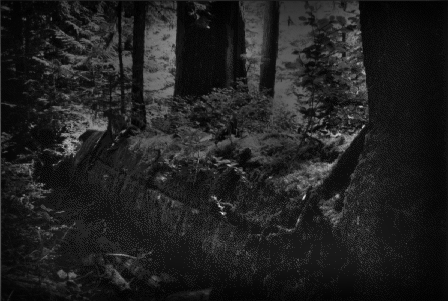
\includegraphics{pics/resulting_image.png}
			\caption{The result}
			\label{fig:result}		
		\end{figure}
							    
		\subsection{Experiments with different images}
		If homomorphic filtering is applied on images with a more appearent
		illumination distortion, such as figure~\ref{fig:gamma_diff} taken
		\begin{figure}[h!]
        \centering
		\begin{subfigure}[b]{0.5\textwidth}
                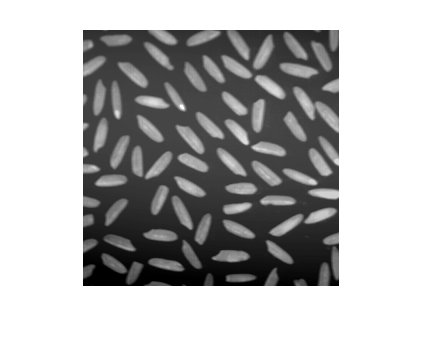
\includegraphics[width=\textwidth]{pics/microbes_before.png}
                \caption{Original image}
                \label{fig:microbe_before}
        \end{subfigure}%
        \begin{subfigure}[b]{0.5\textwidth}
                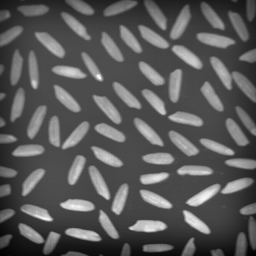
\includegraphics[width=\textwidth]{pics/microbes_after.png}
                \caption{Image after homomorphic filtering}
                \label{fig:microbe_after}
        \end{subfigure}
        \caption{An image with a appearent illumination distortion in the background}	
        \label{fig:gamma_diff}
		\end{figure}
		from the matlab image processing toolbox, the effects are much more obvious. 
		In this image there is a large illumination
		distortion in the background (the black gradient), which here is efficiently 
		removed by the homomorphic filtering process (the black, uniform gradient border
		comes from the zero padding). \\
		\\
		When reading various papers on the
		subject we found several other areas where homomorphic filtering is very effective,
		such as a preprocessing step for facial recognition. The human face has many convex
		portions, which contributes to illumination. In the paper~\cite{Fan20111468}, HF
		is used to remove this illumination and bring forth the edges in the face, making
		the facial recognition algorithms perform better under varying lightning conditions.
		%Elaborate perhaps?
% \end{document} 
